
\chapter{Introduction}
\label{chapter1}

% 1.1.
\section{Plasma Science}

This thesis is multidisciplenary by nature, incorporating aspects of mathematics, physics and computer science throughout 
the various challenges faced in reaching the conclusions we have. 


Before burying ourselves in the thick of our results we 
will cover the requisite knowledge for working in the plasma science simulation space. First we'll discuss what 
the physical object of our attention (``plasma'') actually is, with a brief discussion on the design of fusion reactors, where we will 
emphasise the structures that specifically relate to our interests. In the background chapter we will expound on this by 
building the mathematical theory underpinning physical processes within the fusion reactor, providing us a way to reason
about the behaviour of plasma (and related processes) inside a fusion reactor, or, more accurately, approximate their behaviour 
via simulation.




% 1.1.1.
\subsection{I'm a Mathematician... what is ``plasma''?}

While an initially daunting topic, fear not fearful mathematician, for many of the inherently physical 
behaviours in plasma science we require can be expressed in terms of our dearest mathematical expressions -- differential equations! 
But first, what actually is ``plasma''? Webster's dictionary defines plasma to be ``a green faintly translucent quartz'' \cite{websters_plasma}. 
While I'm sure there isn't no relation between crystals and our investigations, this is unfortunately, not the recipient of our affection. 

When plasma is referred to in everyday conversation it is often noted as being the ``4th state of matter''. To introduce slightly more rigour,
plasma is an extension of the gaseous state of matter, where its energy (read: temperature) is increased sufficiently high that the electrons 
are no longer bound by the electromagnetic force to the atom's nucleus \red{REFERENCE}. The resulting substance is a ``pool'' of cations (the positively charged nuclei), and 
electrons (negatively charged), that exhibits interesting properties. It is these properties that we seek to exploit in the search of controlled, 
sustained fusion reactions.

Plasma is abundant in nature -- just not in many places that we as Humans commonly look. Stars are the most immediate example of matter in a plasma state, 
and are readily viewable (at least for half the day). Lightning strikes are paths through the atmosphere which are ionised, 
and neon signs work by heating Neon gas within a tube to ionise it \red{REFERENCE}.

The question then is, what is ``fusion'', and how does this relate to plasma? The answer comes back to energy. Analogously to a fission reaction, 
where energy is released through the division of atoms, one can also fuse two separate atoms together and have large amounts of energy emitted 
as a bi-product of that fusion. It is (essentially) this extra energy that we wish to harness when harvesting energy from a fusion reactor.

While there are no shortages of elements that can theoretically be used to fuel a fusion reactor, the one most commonly associated with fusion is Deuterium -- a stable isotope of Hydrogen that 
has a neutron in its nucleus (whereas a 'standard' Hydrogen atom contains only a single proton). Analogously, Tritium is an isotope of Hydrogen
that has two neutrons in its nucleus (though is much less stable). Consider the fusion of a Deuterium atom with a Tritium atom:
\[ \prescript{2}{}{\text{H}} + \prescript{3}{}{\text{H}} \stackrel{\text{(fusion)}}{\to} \prescript{4}{}{\text{He}} + n + 17.59 \, \text{MeV} \]

Here two Hydrogen isotopes fuse together to form a single Helium-$4$ atom, and in the process of doing so release 
a single neutron and $17.59$ MeV of energy. This excess energy is what is so attractive about fusion processes as a sustainable 
energy source -- for such little input we receive a substantial amount of energy, and at that, using one of the most abundant 
resources available on Earth; water.

The question then becomes, how do we drive this fusion process? If two atoms can fuse as such, why do we not 
see atoms fusing everywhere around us accompanied by violent explosions destroying all that we've 
come to know and love? The answer is that we kind of do -- just not normally in the places that humans expect to be inhabiting. In fact, we see this happening everyday --
for those of us fortunate enough to be able to see the sun that is. Our sun 
is a large ball of plasma where an estimated $9.3 \times 10^{37}$ fusion reactions are expected to occur every second \cite{nasa-sun-fusion}, 
and is one of the easiest examples of both plasma as a state of matter, and of a self-sustaining fusion reaction.

How then do two hydrogen atoms fuse -- how can we create a sun on Earth? The nucleus of an atom (consisting of positively charged 
protons, and neutral neutrons) is positively charged, and so two atoms' nuclei will repel each other due to the Coulomb force when pushed together. This is the force 
we have to overcome to enable a fusion reaction to take place (and what stops the world around us burning!). To overcome this the process is relatively ``simple'' -- 
we just increase the energy of our atoms so that when they collide they collide with enough energy to overcome this force, allowing the strong force to become
dominant, fusing the two atoms. When we energise a mass (take a gas here) of atoms enough, they become ionised however, which is 
exactly the state of plasma we described earlier. In other words, if we want to reason about the creation, sustainment, and effects of 
fusion reactions, we need first to understand the dynamics of plasma, the medium in which the fusion reactions take place. From this comes a plethora of questions, ranging from 
``how do we generate such a plasma?'' to ``how do we reliably control such a plasma'' and ``how do we harness such a plasma''? Alas, we 
digress however, as we do not seek to solve the big problems in fusion science in this here mere mortal thesis. Instead, now equipped 
with at least a passing knowledge of what constitutes a ``plasma'' state and what it means for a fusion reaction to take place, 
we will humbly delve into the inner workings of fusion reactor terminology and design.


% 1.1.2.
\subsection{Fusion Reactor Design 101}

Here we will discuss the important structural aspects of a Tokamak fusion reactor. The term ``Tokamak'' is a 
Russian acronym which translates as ``toroidal chamber with magnetic coils'' \cite{iter-tokamak-acronym}. Aptly, a Tokamak is a toroidal 
object which is used as a vessell for plasma which is driven via external magnetic coils. 





In reality, reactors do not often have such nice geometry. Figure \ref{fig:east-geometry}
\begin{figure}[h!]
    \centering
    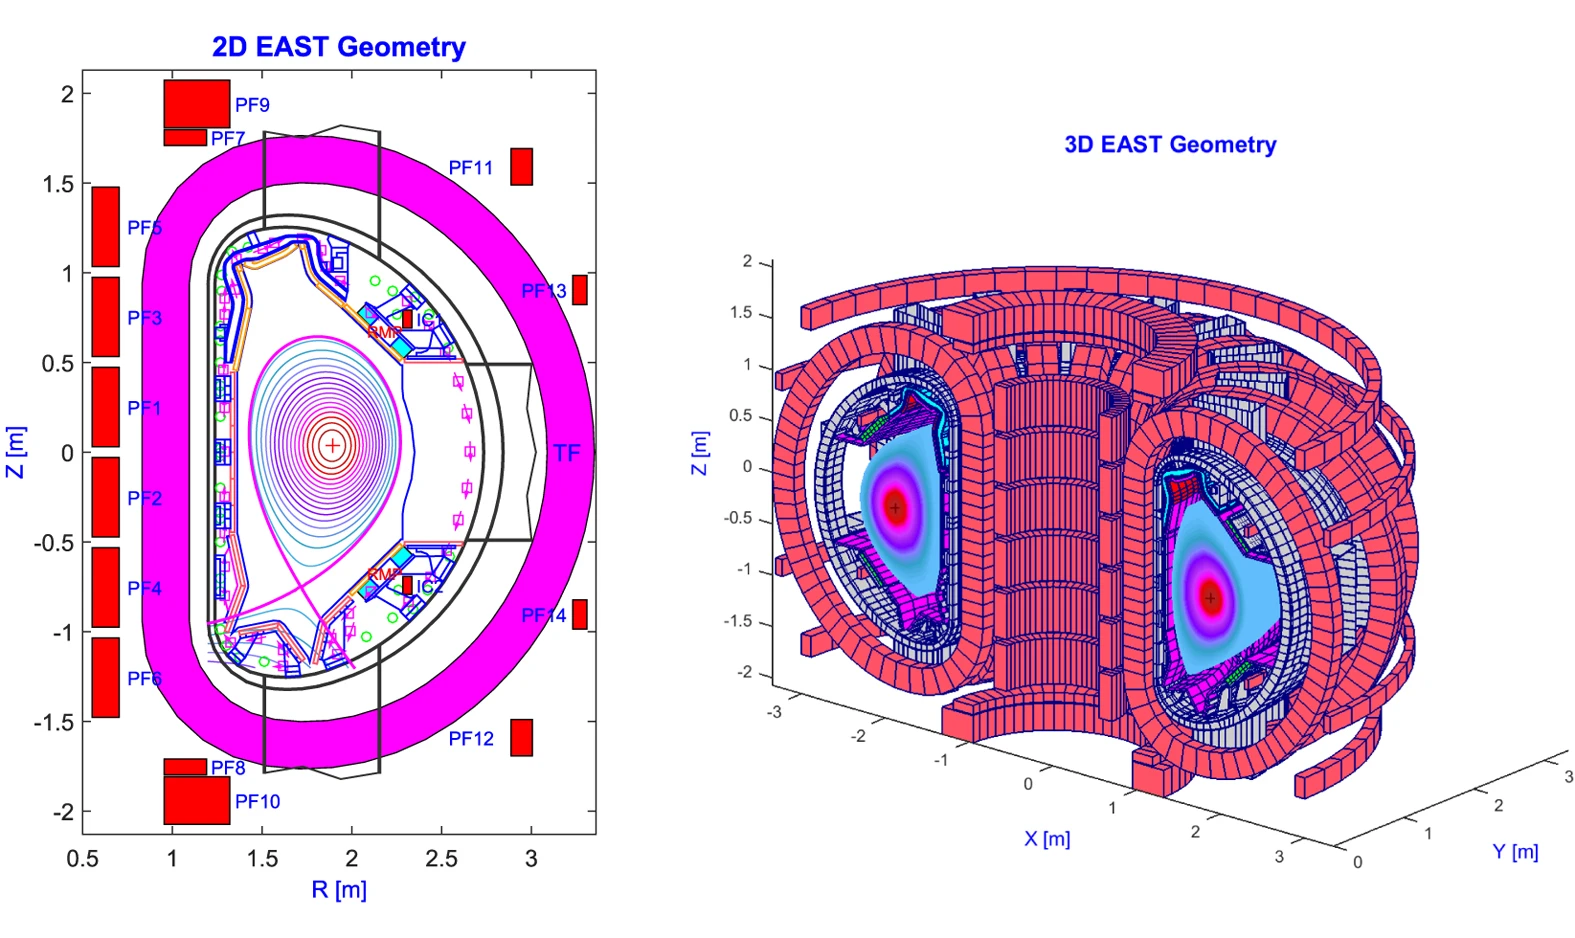
\includegraphics[scale=0.2]{imgs/c1/east-cross-section.png}
    \caption{EAST fusion reactor geometry. This is a 3D model of its cross section, highlighting the irregular shape}
    \label{fig:east-geometry}
\end{figure}

Diagram

Poloidal vs toroidal flux

Magnet positioning

Heating of plasma

Confinement

REs

% 1.2
\section{What problem does this thesis address?}

Talk about paper Matthew and Artur released. Presence of residual REs.

% 1.2.1
\subsection{What results do we seek?}

To provide a theoretical basis for exploring the observed anomalies. 
To see if theory supports the observation

% 1.3.
\section{Project Progression}

Work inspired by Matthew's paper 

First expanded MHD equations linearly with a perturbation treatment

Mathematical PDE theory developed by Wang. Identified errors in paper, fixed. 

Developed a simulation to reproduce results. Then went other direction, 
solving for parameters for data. 

Simulated current inversion.

ISTTOK data matching.

Feasibility



% 1.4.
\section{Structure of Thesis}

TODO (after writing it)

